\documentclass[a4paper, 12pt]{article}

\usepackage{newtxtext} \usepackage{newtxmath}
\usepackage{graphicx}
\graphicspath{ {../Images/} }
\usepackage[utf8]{inputenc}
\usepackage[T1]{fontenc}
\usepackage{textcomp}
\usepackage{amssymb}
\usepackage{amsmath, amssymb}
\newtheorem{problem}{Problem}
\newtheorem{example}{Example}
\newtheorem{lemma}{Lemma}
\newtheorem{theorem}{Theorem}
\newtheorem{problem}{Problem}
\newtheorem{example}{Example} \newtheorem{definition}{Definition}
\newtheorem{lemma}{Lemma}
\newtheorem{theorem}{Theorem}
\usepackage{parskip}

\author{SLP}
\title{Discrete mathematics II : Final exam proofs}

\begin{document}

\maketitle
~ 
~
\begin{center}
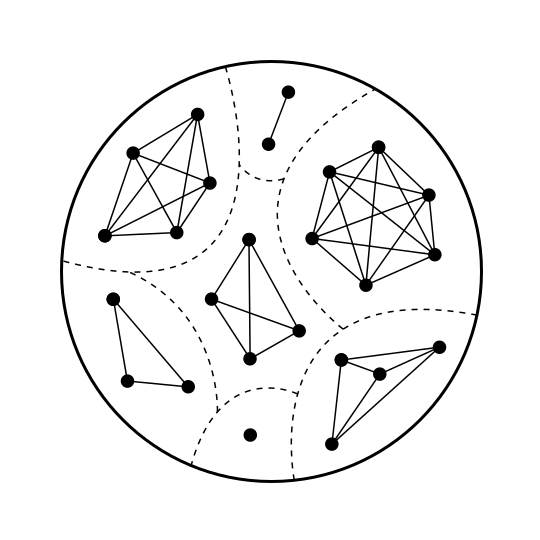
\includegraphics[scale=0.35]{equiv}
\end{center}

\clearpage
\tableofcontents
\clearpage 

\section{Read me}

Most proofs in this document come directly from lectures. A few from PDFs from
previous years. In most cases I assume the reader is familiar with the relevant
definitions---e.g. in proving a problem is NP-complete I do not waste time
reminding him what NP-completeness is---.

This document may contain errors. It will probably contain typing errors,
though I have strived to correct all of them. It will perhaps, though hopefully
not, contain conceptual errors. In short, these are the notes of a student, not
of an expert. Study them with a watchful and critical eye. Should you find an
error, let the author know or send a pull request correcting it. All corrections
are welcome.

~ 




\clearpage 

\section{Baby Brooks}

\begin{quote}
    \textbf{Notational note.} I use $\mathcal{G}$ to denote the Greedy 
    algorithm.
\end{quote}

We wish to prove that if $G = (V, E)$ is connected and non-regular, then
$\chi(G) \leq \Delta$.

Let $x_0 \in V$ be s.t. $d(x_0) = \delta$. Since $G$ is
connected, running BFS from $x_0$ adds all vertices to the BFS tree. Let
$\mathcal{O}^{-1}$ be the ordering of the vertices s.t. $z$ is the $i$th vertex
if it was the $i$th one to be added by BFS. Trivially, $x_0$ is the first
vertex in $\mathcal{O}^{-1}$. Let $\mathcal{O}$ be the reverse order, with
$x_0$ last. We will prove $\mathcal{G}$ colors $G$ with at most $\Delta$ colors
if it uses the ordering $\mathcal{O}$.


Observe that, in the DFS run, every $x \neq x_0$ is inserted by a neighbor that
was already in the tree. In other words, in the $\mathcal{O}^{-1}$ order, every
vertex has a neighbor that precedes him in the order. Consequently, in
$\mathcal{O}^{-1}$, every $x \neq x_0$ has a neighbor that succeeds him in the
order. 

It follows that the worst case scenario for the coloring of $x \neq x_0$ is
that it has $d(x) - 1$ preceding neighbors. $\therefore $ $\mathcal{G}$
eliminates at most $d(x) - 1 \leq \Delta - 1$ colors. Then $x$ can be colored
with a color in $\left\{ 1, \ldots, \Delta \right\} $.

When $\mathcal{G}$ reaches $x_0$ it eliminates at most $d(x_0) = \delta$
colors. Since $G$ is non-regular $\delta < \Delta$.
$\therefore $ There is at least one color for $x_0$
in $\left\{ 1, 2, \ldots, \Delta \right\} $.

\end{quote}
\normalsize

\pagebreak

\section{Max flow, min cut}

Let $f$ a flow over a network $\mathcal{N}$. We want to prove two things:
\textit{(1)} $v(f) \leq Cap(S)$ for any cut $S$ and \textit{(2)} $f$ is maximal
iff there is a cut $S$ s.t. $v(f) = Cap(S)$.

\textit{(1)} We know $v(f) = f(S, \overline{S}) - f(\overline{S}, S)$. Since
$f(A, B)$ is a sum over $f$ and $0 \leq f(\overrightarrow{ab}) \leq
c(\overrightarrow{ab})$ for any $\overrightarrow{ab} \in E$, 

$$v(f) = f(S, \overline{S}) - f(\overline{S}, S) \leq f(S, \overline{S})$$

The same logic implies $f(S, \overline{S}) \leq c(S, \overline{S}) = Cap(S)$.
Then $v(f) \leq f(S, \overline{S}) \leq Cap(S)$. $\blacksquare$

\textit{(2: $\Leftarrow$)} Assume there is a cut $S$ s.t. $v(f) = Cap(S)$. Let
$g$ an arbitrary flow. Then $v(g) \leq Cap(S) = v(f)$. Then $f$ is maximal.
Furthermore, it is trivial by definition of $Cap$ that $Cap(T) \geq v(f)$ for
any cut $T$. Then $Cap(T) \geq Cap(S) \Rightarrow S$ is minimal.

\textit{(2 : $\Rightarrow$)} Assume $f$ is maximal. Let

$$
S = \left\{ s \right\} \cup \left\{ x \in V : \exists f\text{-camino
aumentante entre $s$ y $x$} \right\} 
$$

$S$ is a cut because, if $t \in S$, there is an augmenting path 
$s \ldots t$ and the flow can be augmented, which contradicts 
that $f$ is maximal.

Recall that $v(f) = f(S, \overline{S}) - f(\overline{S},S)$. The first 
term in the difference is

\begin{align*}
    f(S, \overline{S}) &= \sum_{x \in S, z \not\in S, \overrightarrow{xz} \in E}
    f(\overrightarrow{xz})
\end{align*}

Let $\overrightarrow{xz} \in E$ a side in the range of the sum above.
Then there is an augmenting path $s \ldots x$ and there is no 
augmenting path $s \ldots z$. But $\overrightarrow{xz} \in E$ and 
$s\ldots x \ldots z$ is a path. Since it cannot be an augmenting path,
we must have $f(\overrightarrow{xz}) = c(\overrightarrow{xz})$. 
Then $f(\overrightarrow{xz}) = c(\overrightarrow{xz})$ for all $x \in S$, $z
\not\in S, \overrightarrow{xz}\in E$. Therefore

\begin{align*}
    f(S, \overline{S}) = \sum_{\ldots} f(\overrightarrow{xz}) = \sum_{\ldots}
    c(\overrightarrow{xz}) = Cap(S)
\end{align*}

Now consider the second term in the difference:

\begin{align*}
    f(\overline{S}, S) = \sum_{w \not\in S, x \in S, \overrightarrow{wx} \in E}
    f(\overrightarrow{wx})
\end{align*}

Let $\overrightarrow{wx}$ an arbitrary side in the sum above. Again,
there must be an augmenting path $s \ldots x$, but not one 
$s \ldots w$. But $\overrightarrow{wx}$ is a side, and then 
$s \ldots \overleftarrow{xw}$ is not augmenting only if 
$f(\overleftarrow{xw}) = 0$. This means $f(\overrightarrow{wx}) = 0$
for all $\overrightarrow{wx}$ in the range of the sum above.

$\therefore $  $v(f) = Cap(S) - 0 = Cap(S)$. $\blacksquare$

\pagebreak

\section{Edmond-Karp}

Primero, recordemos algunas definiciones: 

\begin{itemize}
    \item \textit{Cut :} A cut is a set $S \subseteq V$ s.t. $s \in S, t
        \not\in S$. A theorem establishes that $v(f) \leq CAP(S)$ for any cut
        $S$. If $CAP(S) = v(f)$, we say $S$ is minimal. 
\end{itemize}

Furthermore, if $v(f) = CAP(S)$, then $f$ is maximal and $S$ is minimal. And if $f$ is maximal,
necessarily there is some $S$ s.t. $v(f) = CAP(S)$.

\subsection{Complexity}

Edmond-Karp runs BFS $\zeta$ times to find the $f$-augmenting path. At the end
of each run, it updates the flow. Each BFS run has complexity $O(\sum_{x \in V}
d(x)) = O(2m) = O(m)$. Updating the flow has a complexity $O(n)$ because the
$f$-augmenting path is of length at most $n$. Then the complexity is $\zeta
\left( O(m) + O(n) \right) = \zeta O(m)$. 

$\zeta$ is bounded by the number of $f$-augmenting paths that can be found.
This number is $m \times \varphi$, where $\varphi$ is the number of times a
side can become critical. Let us determine $\varphi$.


Let $f_0, f_1, f_2, \ldots$ the flows obtained over the iterations of E.K. Let
$\overrightarrow{xy}$ a side that becomes critical at iteration $k$. Then
either it saturated being forward, or it emptied being backward. Let us look at
each case.

\textit{Case 1: It saturated being forward.}

\textit{(1.1)} Assume it saturated being forward. Then a $f_k$-augmenting path of
the form $s \ldots \overrightarrow{xy} \ldots t$ was found. Since we are using
E.K., this path is of minimal length, which means $d_k(y) = d_k(x) + 1$.

\textit{( 1.2 )} Assume $\overrightarrow{xy}$ becomes critical again 
at some iteration $j > k$. There are two options: it emptied because 
$\overrightarrow{yx}$ was used backwardly in the iteration, or it 
saturated again because, in some iteration $i \in (k, j)$, a fraction
of the flow was returned backwardly. In both cases, there is a $i \leq k$ s.t.
a $f_i$-augmenting path of the form $s \ldots \overrightarrow{yx} \ldots t$ was
found. Since we are using E.K., this path is of minimal length, 
and $d_i(x) = d_i(y) + 1$.

\textit{(1. 3)} Because the length of the augmenting paths 
never decreases across iterations, $d_j(t) \geq d_i(t) = d_i(x) + b_i(x)$.
This means 

    \begin{align*}
        d_j(t) \geq d_i(y) + 1 + b_i(x) \geq d_k(y) + 1 + b_k
    \end{align*}

But $d_k(y) = d_k(x) + 1$. Then

    \begin{align*}
        d_j(t) \geq d_k(x) + 1 + 1 + b_k(x) = d_k(t) + 2
    \end{align*}

\textit{Case 2: It emptied being backwards}

\textit{(1.1)} Assume $\overrightarrow{xy}$ empties. Then the $f_k$-augmenting 
path is of the form $s \ldots \overrightarrow{yx} \ldots t$ with 
$d_k(x) = d_k(y) + 1$.

\textit{(1.2)} Assume it becomes critical again at iteration $j$.
Then it is either saturated or emptied again. In both cases, 
some iteration $i \leq j$ must find the $f_i$-augmenting path 
$s \ldots \overrightarrow{xy} \ldots t$ and therefore 
$d_i(y) = d_i(x) + 1$. 

\textit{(1.3)} We know $d_j(t) \geq d_i(t)$. But

    \begin{align*}
               &=d_i(y) + b_i(y) \\ 
               &= d_i(x) + 1 + b_i(y) \\ 
               &\leq d_k(x) + 1 + b_k(y) \\ 
               &= d_k(y) + 1 + 1 + b_k(y) \\ 
               &=d_k(t) + 2
    \end{align*}

Then $d_j(t) \geq d_k(t) + 2$.

\textit{Conclusion.} Once a side $\overrightarrow{xy}$ becomes 
critical, the length of the augmenting paths found 
must increase at least by two before it can become 
critical again. Then a side can become critical 
at most $\varphi = \frac{n}{2} = O(n)$ times. Then 
the complexity of Edmond-Karp is $(\varphi \times m) \times O(m) = O(nm^2)$.
    

\pagebreak 

\subsection{Augmenting paths are non-decreasing}

Let $A = \left\{ x \in V : d_{k+1}(x) < d_k(x) \right\} $ and
assume $A \neq \emptyset$. Let $x_0 \in A$ be the vertex whose distance
$d_{k+1}(x_0)$ from $s$ is minimal; i.e. $d_{k+1}(x_0) \leq d_{k+1}(y) ~
\forall y \in A$. Since $x_0 \in A$, $d_{k+1}(x_0) < d_k(x_0) \leq \infty$.
Then there exists a $\mathcal{P}_{k+1} = s \ldots x_0$ of minimal length.
Let $z$ be the predecessor of $x_0$ in this path.

By definition of $d_f$, the length of the path is $d_{k+1}(x_0)$. Because the
path is of minimal length to $x_0$, it is of minimal length to any predecessor
of $x_0$ in it, including $z$. Then $d_{k+1}(z) = d_{k+1}(x_0) - 1$. This
implies $z \not\in A$.

There are two possible cases: either $\overrightarrow{xz} \in E$
or $\overrightarrow{zx} \in E$.

\textit{(Case 1):} If $\overrightarrow{zx_0} \in E$, then
$d_{k+1}(z) < d_{k+1}(x_0)$. Since $z \not\in A$,

\begin{align*}
    d_k(z) \leq d_{k+1}(z) < d_{k+1}(x_0) < \infty
\end{align*}

Since $d_k(z) < \infty$, there is an $f_{k}$-augmenting path from $s$ to $z$.
Then, in principle, $s \ldots z x$ could be  an augmenting path. But
if this were the case, 

$$d_k(x_0) \leq d_k(z) + 1 \leq d_{k+1}(z) + 1 = d_{k+1}(x)$$ 

which implies $x_0 \not\in A$ ($\bot$). $s\ldots zx$ is not $f_k$-a.p. This can
only happen if $f_k(\overrightarrow{zx_0}) = c(\overrightarrow{zx_0})$ (the
side is saturated). Since the side is used in a $f_{k+1}$-a.p. it must be the
case that $f_{k+1}(\overrightarrow{zx_0}) < c(\overrightarrow{zx_0})$. This
means $\overrightarrow{zx}$ was used backwards in the $k$th iteration, or
rather that $f_k = s \ldots \overleftarrow{x_0z} \ldots t$.

Since this is Edmond-Karp, augmenting paths are of minimal length. Then 

\begin{align*}
    d_{k}(z) &= d_k(x_0) + 1   \\ 
             &> d_{k+1}(x_0) + 1 \\ 
             &=d_{k+1}(z) + 2 \\ 
             & \geq d_{k}(z) + 2
\end{align*}

which is absurd.

\textit{1.3.2} If  $\overrightarrow{xz}$ is a side then again

\begin{align*}
    d_k(z) \leq d_{k+1}(z) < d_{k+1}(x_0) < \infty
\end{align*}

Then there is an $f_k$-a.p. $s \ldots z$ and, at least in principle, 
$s \ldots \overrightarrow{zx}$ could also be augmenting. But if this were the case,
we would have 

$$
d_k(x_0) = d_k(z) + 1 \leq d_{k+1}(z) + 1 = d_{k+1}(x_0) 
$$

which would imply $x_0 \not\in A$ ($\bot$). Then $s \ldots \overrightarrow{zx_0}$ is 
not augmenting, which means the side $\overrightarrow{x_0z}$ cannot 
be used backwards. This can only be true if $f_k(\overrightarrow{x_0z} = 0$.
But since the side is used backwards in the $f_{k+1}$-augmenting path,
it must be used forward in this iteration. Which means $s \ldots \overrightarrow{x_0z} \ldots t$
is augmenting. But then 

\begin{align*}
    d_{k}(z) &= d_{k}(x_0) + 1 \\ 
             &> d_{k+1}(x_0) + 1 \\ 
             &= d_{k+1}(z) +2 \\ 
             &\geq d_{k}(z) + 2 
\end{align*}

which is absurd.

\textit{Conclusion.} In both cases a contradiction arises. The contradiction
comes from assuming $A \neq \emptyset$. Then $A = \emptyset$. $\blacksquare$


\pagebreak

\section{Complexity of Dinitz}


We will prove the complexity of Dinitz is $O(n^2m)$.

Let $\psi$ the complexity of finding a blocking flow and $\varphi$ the
complexity of building an auxiliary network. We know the level $t$ in the
auxiliary networks is increasing, which implies there are at most $n$ auxiliary
networks. $\therefore $ The complexity of Dinitz is $\left( \psi + \varphi
\right) O(n) $.

Since we use DFS, $\varphi = O(m)$. Let us prove $\psi = O(nm)$. If we can
prove this, we will have the overall complexity $\left( O(nm) + O(m) \right)
O(n) = O(n^2m) $, which is what we want.

\textbf{Original algorithm.} In this version, the auxiliary network is s.t. all
vertices have an exiting edge. This means DFS always reachs $t$ without need to
backtrack. Then DFS is not $O(m)$ but $O(N) = O(n)$, where $N$ is the number of
levels in the auxiliary network.

Every path deletes at least one edge from the auxiliary network. $\therefore $
There are $O(m)$ paths.  $\therefore $ the complexity of finding the 
paths and updating the flow with them is $O(nm)$. But there is 
an extra cost associated to the property that all vertices have an 
exiting edge.

To enforce this invariant, Dinitz used the pruning operation (\textit{podar}).
Pruning goes from high- to low-level vertices and deletes the sides that have
no exiting edge. Checking if a vertex has an exiting edge is $O(1)$; there are
$O(n)$ vertices and one pruning operation per path; there are $O(m)$ paths.
$\therefore $ Pruning so far is $O(mn)$.

But erasing the vertices has some complexity. This is done at most once per
vertex, and it is likely that once we prune one vertex, pruning the following
ones is less complex (because we are removing edges). So we will calculate the
\textit{average} complexity, not the worst-case complexity, of the problem.

Deleting a vertex $x$ and its edges is $O(d(x))$; over all vertices this gives
$\sum O(d(x)) = O(m)$ (Handshaking Lemma).  $\therefore $ $\psi = O(nm) + O(nm)
+ O(m)= O(nm)$.

$\therefore $ The complexity of Dinitz is $\left( O(nm) + O(m) \right)O(n) = O(n^2m) $

\textbf{Western version.} The simplest approach is to give the pseudo-code. We
are speaking of finding a blocking flow in the auxiliary network, do not think
we are talking of the original network.

\begin{align*}
    &g := 0 \\ 
    &\textbf{bool } flag := \textbf{true} \\ 
    &\textbf{while } flag ~ \textbf{ do} \\ 
    & ~ ~ ~ ~ \textbf{type } path := [s] \\ 
    & ~ ~ ~ ~ \textbf{int } x := s \\ 
    & ~ ~ ~ ~ ~ ~ ~ ~ \textbf{while } x \neq t \textbf{ do } \\ 
    & ~ ~ ~ ~ ~ ~ ~ ~ ~ ~ ~ ~ \textbf{if } \Gamma^{+}(x) \neq 0 \textbf{ then } \\ 
    & ~ ~ ~ ~ ~ ~ ~ ~ ~ ~ ~ ~ ~ ~ ~ ~ ~ \text{tomar } y \in \Gamma^{+}(x) \\ 
    & ~ ~ ~ ~ ~ ~ ~ ~ ~ ~ ~ ~ ~ ~ ~ ~ ~ \text{agregar } y \text{ a } path \\ 
    & ~ ~ ~ ~ ~ ~ ~ ~ ~ ~ ~ ~ ~ ~ ~ ~ ~ x := y &\left\{ \text{Esta línea y la anterior son la parte (A) de avanzar} \right\}  \\ 
    & ~ ~ ~ ~ ~ ~ ~ ~ ~ ~ ~ ~ \textbf{else }  \\ 
    & ~ ~ ~ ~ ~ ~ ~ ~ ~ ~ ~ ~ ~ ~ ~ ~ \textbf{if } x \neq s \textbf{ then }  &\left\{ \text{(R) Retroceder} \right\} \\ 
    & ~ ~ ~ ~ ~ ~ ~ ~ ~ ~ ~ ~ ~ ~ ~ ~ ~ ~ ~ ~ z := \text{elemento anterior a $x$ en  } path  \\ 
    & ~ ~ ~ ~ ~ ~ ~ ~ ~ ~ ~ ~ ~ ~ ~ ~ ~ ~ ~ ~ \text{borro } x \text{ de } path\\ 
    & ~ ~ ~ ~ ~ ~ ~ ~ ~ ~ ~ ~ ~ ~ ~ ~ ~ ~ ~ ~ \text{borro } \overrightarrow{zx} \text{ de la n.a.}\\ 
    & ~ ~ ~ ~ ~ ~ ~ ~ ~ ~ ~ ~ ~ ~ ~ ~ ~ ~ ~ ~ x := z\\ 
    & ~ ~ ~ ~ ~ ~ ~ ~ ~ ~ ~ ~ ~ ~ ~ ~ \textbf{else }   \\ 
    & ~ ~ ~ ~ ~ ~ ~ ~ ~ ~ ~ ~ ~ ~ ~ ~ ~ ~ ~ ~ flag := 0   \\ 
    & ~ ~ ~ ~ ~ ~ ~ ~ ~ ~ ~ ~ ~ ~ ~ ~\textbf{fi} \\ 
    & ~ ~ ~ ~ ~ ~ ~ ~ ~ ~ ~ ~ \textbf{fi}\\
    & ~ ~ ~ ~ ~ ~ ~ ~ \textbf{od } \\
    & ~ ~ ~ ~ ~ ~ ~ ~ \textbf{if } x = t \textbf{ then } &\left\{ \text{(I) Incrementar} \right\}  \\ 
    & ~ ~ ~ ~ ~ ~ ~ ~ ~ ~ ~ ~ \text{aumentar flujo $g$ a lo largo de } path \\
    & ~ ~ ~ ~ ~ ~ ~ ~ ~ ~ ~ ~ \text{borrar lados saturados} \\ 
    & ~ ~ ~ ~ ~ ~ ~ ~ \textbf{fi}\\
    &\textbf{od}
\end{align*}

Let $\Sigma = \left\{ A, I, R \right\} $. A Dinitz run (in the Western version)
is a word $w \in \Sigma^{*} $. Consider all  over this language of the form $A
\ldots AX$ with $X \in \Sigma$, $X \neq A$. Each $A$ is $O(1)$;
each $R$ is $O(1)$; each $I$ is traversing the path twice, once to update the flow,
once to erase the edges $\Rightarrow$ $I$ is $O(n)$.

Each $A$ moves the pivot $x$ from one level to the next. $\therefore $ There 
are $O(n)$ letters $A$ in the word. 

\begin{align*}
    \therefore \qquad &(1) O(A \ldots A R) &= O(n) + O(1) + O(n) \\ 
               &\textit{(2)} O(A \ldots AI) &= O(n)(\#A) + O(n)(\#I) = O(n)
\end{align*}

Each $R$ deletes an edge and each $R$ deletes \textit{at least} an edge.
$\therefore $ There are $O(m)$ words of the form $A\ldots AX$.$\therefore $ The
total complexity is $O(nm)$.




\pagebreak

\section{Codes}

\subsection{Hamming bound}

\begin{quote}
\begin{theorem}[Cota de Hamming]
    Sea $C \subseteq \left\{ 0, 1 \right\}^n $. Sea $\delta = \delta(c)$ y $t =
    \left\lfloor \frac{\delta-1}{2} \right\rfloor$. Entonces 

    \begin{align*}
        |C| \leq \frac{2^n}{1 + n + \binom{n}{2} + \ldots  + \binom{n}{t}}
    \end{align*}
\end{theorem}


    \begin{definition}[Disco]
        The disk of radius $r$ around $\alpha \in \left\{ 0, 1 \right\}^n $ is
    
        \begin{align*}
            D_r(\alpha) = \left\{ \gamma \in \left\{ 0, 1 \right\}^n : d_H(\alpha, \gamma) \leq r  \right\} 
        \end{align*}
    \end{definition}
\end{quote}

Let $A = \bigcup_{v \in C} D_t(v)$. Since $C$ corrects $t$ errors, for any two 
different words $v, w \in C$,$ D_t(v) \cap D_t(w) = \emptyset$. This means $A$
is a disjoint union. $\therefore $ $|A| = \sum_{v \in C} |D_t(v)|$.

Let $S_r(v) = \left\{ w \in \left\{ 0, 1 \right\}^n : d_H(v, w) = r \right\} $.
Then $D_t(v) = \bigcup_{r=0}^{t}S_r(v)$, and this union is trivially disjoint.
Then $|D_t(v)| = \sum_{r = 0}^{t} |S_r(v)|$. The question is what is the value
of $|S_r(v)|$.

Recall that

\begin{align*}
    w \in S_r(v) &\iff d_H(v, w) = r \\ 
          &\iff w \text{ differes by $r$ bits from } v
\end{align*}

In other words, each $w \in S_r(v)$ is fully determined by the 
bits which makes it different from $v$, and this set of bits 
fully determine $w$. This means there is a bijection $\psi : S_r(v) \to B$ where 
$B$ is the set of all subsets of $r$ bits from a set of $n$ bits.
set of all subsets of $r$  bits from a set of $n$ bits.

Because it is a bijection,


\begin{align*}
    |S_r(v)| &= |B| = \binom{n}{r}
\end{align*}

This means

    \begin{align*}
        |D_t(v)| &= \sum_{r=0}^{t} |S_r(v)| \\ 
                 &= \sum_{r=0}^{t} \binom{n}{r}
    \end{align*}

By definition of $A$,

    \begin{align*}
        |A| &= \sum_{v \in C} \left( \sum_{r=0}^{t} \binom{n}{r} \right) \\ 
            &= |C| \sum_{r=0}^{t} \binom{n}{r}\\
        \Rightarrow |C| &=  \frac{|A|}{\sum_{r=0}^{t} \binom{n}{r}}
    \end{align*}

    Since $A \subseteq \left\{ 0,1 \right\}^n \Rightarrow |A| \leq 2^n $, 

    \begin{align*}
        |C| \leq \frac{2^n}{\sum_{r=0}^{t} \binom{n}{r}}
    \end{align*}

\pagebreak


\subsection{$\delta(C) = \min \left\{ j : \exists S \subseteq H_{*n} : |S| = j \land  S \text{ is LD} \right\} $}

\begin{quote}
    \textbf{Notation.} I use $H_{*n}$ to denote the set with the $n$ columns
    of $H$. I use $H^{(i)}$ to denote the $i$th column of $H$.
\end{quote}

Let $s = \min \left\{ j : \exists S \subseteq H_{*n} : |S| = j \land  S \text{
is LD} \right\} $. This implies there are $s$ columns $H^{(j_1)}, \ldots,
H^{(j_s)}$ s.t. $\sum x_i H^{( j_i )} = 0$ for $x_1, \ldots, x_s$ not all null.

\textit{(1)} Let $w := \sum x_i e_{j_i}$ where $e_{k}$ is the vector with all
zeroes except at the $k$th coordinate. Since not all $x_i$ are zeroes, $w \neq
0$. Now, 

\begin{align*}
    Hw^t &= H \left( x_1 e_{j_1} + \ldots + x_s e_{j_s} \right)^t \\ 
         &= x_1 H e_{j_1}^t + \ldots + x_s H e_{j_s}^t \\ 
         &= \sum x_i H^{(j_i)} &\left\{ \text{Because } He_j^t = H^{(j)} \right\}  \\ 
         &= 0
\end{align*}

Then $w \in Nu(H) = C$. But $|w| \leq s$ and $w \neq 0$. We know $\delta = \min
\left\{ |x| : x \in C, c \neq 0 \right\} $.

$\therefore ~ \delta \leq |w| \leq s$.

\textit{(2)} Let $v \in  C$ s.t. $\delta = |v|$. Then there are 
$i_1, \ldots, i_{\delta}$ s.t. $v = e_{i_1} + \ldots + e_{i_\delta}$.
Since $v \in  C, Hv^t = 0$, which using the same 
logic as before gives $\sum H^{(i_j)} = Hv^t = 0$.

This implies $\left\{ H^{(i_1)}, \ldots, H^{(i_{\delta})} \right\} $ is LD.

$\therefore  s \leq \delta$.

\textit{(3)} Points \textit{(1)} and \textit{(3)} imply $s = \delta$.





\pagebreak

\section{Matchings}

\subsection{Konig}

We want to prove that any bipartite and regular graph $G = (V, E) $ has a
perfect matching. Let $X, Y$ be the two parts of $G$. For any $W \subseteq V$
let $E_W := \left\{ wu \in E : w \in W \right\} $.

\textit{(1)} Let $S \subseteq X$ and $l \in E_S$. It follows that

\begin{align*}
    \exists x \in S, y \in Y : l = xy = yx 
\end{align*}

$\therefore y \in \Gamma(x)$. And since $x \in  S$ we have $y \in \Gamma(S)$ 
and $l \in E_{\Gamma(S)}$.

$\therefore $ $E_S \subseteq E_{\Gamma(S)}$ and $|E_S| \leq |E_{\Gamma(S)}|$.

\textit{(2)} Let us calculate $|E_W|$ when $W \subseteq X$.

Observe that $E_W = \bigcup_{w \in W} \left\{ wv : v \in \Gamma(w) \right\} $.
Furthermore, the union is disjoint, because $wv \in E_W \Rightarrow w \in X
\Rightarrow v \in Y$. Then

\begin{equation*}
    |E_W| = \sum_{w \in W} |\Gamma(w)| = \sum_{w \in W} d(w)
\end{equation*}

Since $G$ is regular, $d(w) = \delta = \Delta$. 

$\therefore $ $|E_W| = \Delta |W|$

\textit{(3)} Using what we established in \textit{(1)}, it follows from \textit{(2)} that

\begin{equation*}
    |S| \Delta \leq |\Gamma(S)| \Delta \Rightarrow |S| \leq |\Gamma(S)| 
\end{equation*}

This holds for any $S \subseteq X$. Then Hall's theorem implies there is a
complete matching from $X$ to $Y$. To prove it is perfect, we must prove $|X| =
|Y|$.

But since $X, Y$ are the two parts of $G$, $E = E_X = E_Y$. Then $|E_X| =
|E_Y|$, which implies $|X| \Delta = |Y| \delta \Rightarrow |X| =
|Y|$.

Alternatively, since there is a complete matching from $X$ to $Y$, $|X| \leq
|Y|$. But the choice of $X$ over $Y$ was arbitrary, and then the same holds for
$Y$. Then $|X| = |Y|$.

In both caes the matching is perfect.



\pagebreak 

\subsection{Hall}

Let $G = (V, E)$ a bipartite graph with parts $X$ and $Y$, and let $Z \in
\left\{ X, Y \right\} $. We want to prove that there is a complete matching
from $X$ to $Y$ iff $\forall S \subseteq Z : |S| \leq |\Gamma(S)| $.

$(\Rightarrow)$ The proof is trivial, because if such matching exists, it
induces an injective function $f : X \to Y$ s.t. $f(x) \in \Gamma(x)$. Since it
is an injection, $|f(S)| = |S|$ for any $S$. Then $f(S) \subseteq \Gamma(S)
\Rightarrow |S| \leq |\Gamma(S)|$.

$(\Leftarrow)$ Assume the Hall condition $|S| \leq |\Gamma(S)|$ holds. Assume
that, after running the algorithm to find a maximal matching, an incomplete
matching is found. We will build $S \subseteq X$ that violates our assumption
(we could use $S \subseteq Y$ without loss of generality).

\textit{(1)} Let $S_0$ be the set of rows unmatched and $T_1 = \Gamma(S_0)$.
Observe that, by assumption, $S_0 \neq \emptyset$, and all columns in $T_1$
have a match that is not in $S_0$. Let $S_1$ the set of rows matching columns
of $T_1$ and $T_2 = \Gamma(S_1) - T_1$. Generally, 

\begin{align*}
    S_i &= \text{Rows matching with } T_i \\ 
    T_{i+1} &= \Gamma(S_i) - \bigcup^{j=i}_{j=0} T_j
\end{align*}

The algorithm stops only when it is revising a row and this row has no
available neighbors; this is, it only stops passing from a $S_i$ to a $T_{i+1}$
when $T_{i+1} = \emptyset$. Furthermore, since each column only labels a single
row (that of its match), and $T_i$ "creates" $S_i$, we have $|S_j| = |T_j|$. 

Define $S = \bigcup S_i, T = \bigcup T_i$, and note that all the $S_i$ are
disjoint and all the $T_i$ are disjoint. Then

\begin{align*}
    |S| &= \sum |S_i| \\ 
        &= |S_0| + \sum |T_i| \\ 
        &= |S_0| + |T|
\end{align*}

$\therefore ~ |S| > |T|$ (since $S_0 \neq \emptyset$).

We must only prove now that $T = \Gamma(S)$. 

\textit{(1)} $T$ are the labeled columns, and each column is labeled by a row in $S$.
Each row only labels its neighbors. This implies $T \subset \Gamma(S)$.

\textit{(2)} Assume $y \in \Gamma(S)$ and $y \not\in T$. Then $y$ was 
not labeled. But since $y \in \Gamma(S)$ there is an 
$x \in S$ s.t. $y \in \Gamma(x)$. Then each time 
the algorithm passes through $x$ it should label 
$y$, which contradicts the fact that $y$ is not 
labeled. Then $y \in T$. Then $\Gamma(S) \subseteq T$.

$\therefore \Gamma(S) = T$ and $|S| > |\Gamma(S)|$. But this contradicts 
the hypothesis that the Hall condition holds. The 
contradiction comes from assuming there wasn't a 
complete matching. $\therefore $ There is a complete
matching. $\blacksquare$

\pagebreak
\section{P-NP}

\subsection{2-Color is polynomial}

We must give a polynomial algorithm that decides whether an arbitrary $G = (V,
E)$ is $\chi(G) = 2$. 

\begin{align*}
    &n\_colored := 0 \\ 
    &\textbf{while } j < n \textbf{ do }\\ 
    &\qquad x := v \in V, v \text{ not colored} \\ 
    &\qquad C(x) := 1 \\ 
    &\qquad n\_colored :=  n\_colored + 1 \\ 
    & \qquad Q = \text{queue with only } x \\ 
    & \qquad\textbf{while } Q \neq \emptyset \textbf{ do } \\ 
    & \qquad \qquad p := pop!(Q) \\ 
    & \qquad \qquad \textbf{for } w \in \Gamma(p) \textbf{ do } \\ 
    & \qquad\qquad\qquad \textbf{if } w \text{ is not colored } \textbf{do} \\ 
    & \qquad\qquad\qquad\qquad push!(w, Q) \\ 
    & \qquad\qquad\qquad\qquad C(w) = 3 - C(p) \\ 
    & \qquad\qquad\qquad\qquad n\_colored = n\_colored + 1 \\ 
    & \textbf{for } \left\{ v, w \right\} \in  E \textbf{ do }\\ 
    & \qquad\textbf{if } C(v) = C(w) \textbf{ return } False \textbf{ else } \textbf{return } True
\end{align*}

\textbf{Complexity.} The inner \textbf{while} traverses the vertices in the
connected component of $x$, which means the outer \textbf{while} is executed
once per connected component. Furthermore, inside the inner \textbf{while} we
loop through $\Gamma(p)$. Then the complexity of the inner \textbf{while} is 

\begin{align*} O \left[ \sum_{p \in \mathcal{C}(x)} d(p) \right] = O \left[ 2
\times \text{edges in } \mathcal{C}(x) \right]  = O(\# \text{edges in }
\mathcal{C}(x)) \end{align*}

where $\mathcal{C}(x)$ is the connected component of $x$. The \textbf{for} loop
is $O(m)$ of course. $\therefore $ the algorithm is polynomial.

\textbf{Correctness.} It is trivial to note that if the algorithm returns
$True$ then $G$ is $2$-color. Now, assume the algorithm returned $False$. Then
there is some $\left\{ v, w \right\} \in E$ s.t. $C(v) = C(w)$. These belong to
the same connected component.

Let $x$  be the root of this connected component from which the queue was
built. Without loss of generality, assume $v$ entered the queue first. 
Then, when $v$ became the first element in the queue, $w$ must have 
already been in the queue. Otherwise, because they are neighbors, $v$
would have added $w$ with the color $3 - C(v)$, which contradicts the 
hypothesis. Then there is a chain of inclusion in the queue

$$x = v_r \to v_{r-1} \to  \ldots \to v_1 \to  v_0 = v$$
$$x = w_t \to w_{t-1} \to  \ldots \to w_1 \to  w_0 = w$$

Since $v$ came first, we must have $r \leq t$, but since $w$ is the queue when
$v$ is its first element, $t \leq r+1$. Now, since the color depends of the
parity of $r$ and $t$, $C(v) = C(w) \Rightarrow t \equiv r \mod 2$. Then $t =
r$.

Let $k$ the first index s.t. $v_k = w_k$; then we have a path $v \to  v_1 \to
v_k = w_k \to  w_{k-1} \to  w_{k-2} \ldots w$ with $wk + 1$ vertices. But since
$v, w$ are an edge, the graph contains $C_{2k+1}$. $\therefore \chi(G) \leq 3$.




\pagebreak

\subsection{3SAT es NP-Completo}.

Let $B = B_1 \land  \ldots B_m$ an instance of SAT with variables 
$x_1, \ldots, x_n$. We build an instance of $3$-SAT 
by transforming each $B_i$ into an $E_i$ as follows:

\textit{Complete.}

\begin{align*}
E_i = (e_1 \lor  e_2 \lor y_1) \land  (\overline{y_1} \lor  y_2 \lor  e_3) \land  (\overline{y_2} \lor  y_3 \lor  e_4) \lor \ldots (\overline{y_{k-3}} \lor e_{k-1} \lor e_{k})
\end{align*}

We want to prove

\begin{align*}
    \exists \overrightarrow{b} : B(\overrightarrow{b}) = 1 \iff \exists \overrightarrow{\alpha} : \tilde{ B }(\overrightarrow{b}, \overrightarrow{\alpha}) = 1
\end{align*}

\textit{($\Leftarrow$)} Asume $B(\overrightarrow{b}) = 0$. Then
$D_i(\overrightarrow{b}) = 0$ for some $i$. Let 
 $e_1, \ldots, e_k$ be the literals in $D_i$.

If $k = 3$ a contradiction ensues trivially. If $k = 2$, then $D_i = e_1 \lor
e_2$ and then $E_i = (e_1 \lor  e_2 \lor y_1) \land  (e_1 \lor  e_2 \lor
\overline{y_1})$. Since $D_i = 0$, $e_1 \lor  e_2 = 0$ and therefore $e_1 = e_2
= 0$ From this follows  $E_i = y_1 \land \overline{y_1} = 1$. $(\bot)$

If $k = 1$ then $e_1 = 0$ and therefore $E_i = (y_1 \lor  y_2) \land  (y_1 \lor
\overline{y_2}) \land  (\overline{y_1} \lor  y_2) \land  (\overline{y_1} \lor
\overline{y_2}) = 0$. But by assumption $E_i = 1 (\bot)$.

If $k\geq 4$ we must observe that, since $D_i(\overrightarrow{b}) =
0$, we have $e_1 = e_2 = \ldots = e_k = 0$. Then this literals 
are neutral elements in the disjunctions and can be ignored.
Since $E_i(\overrightarrow{b}, \overrightarrow{\alpha}) = 1$, its first term 
is true; in other words, $e_1 \lor  e_2 \lor  y_1 = 1
\Rightarrow y_1 = 1$. In all the following cases (except the last),
$E_i = \overline{y_{i-1}} \lor  y_i$ must be true; this is,
$y_i \Rightarrow y_{i+1}$ is true. But the last term is $\overline{y_{k-3}}$,
which cannot be true because $y_1$ and $ y_1 \Rightarrow y_2 \Rightarrow \ldots
\Rightarrow y_{k-3}$. ($\bot$)

\textit{($\Rightarrow$)} Assume $B(\overrightarrow{b}) = 1$. For $k = 1, k = 2$, define 
$y_i = 0$ for all $i$. $\therefore $ $D_i(\overrightarrow{b}) = 1 \Rightarrow
E_i(\overrightarrow{b}, \overrightarrow{\alpha}) = 1$. For $k = 3$ the result 
is trivial. Let us consider the case $k \geq 4$.

Since $D_i(\overrightarrow{b}) = 1$ is a true disjunction, at least one $e_r$
is true under $\overrightarrow{b}$ . Define the following assignment:

\begin{align*}
    &y_1 = y_2 = \ldots = y_{r-2} = 1 \\ 
    &y_i = 0 \text{ para todos los demás $i$}
\end{align*}

Then

\begin{align*}
    E(\overrightarrow{b}, \overrightarrow{\alpha}) &= \left( e_1 \lor e_2 \lor y_1 \right) &\left\{ \text{True because } y_1 = 1 \right\}  \\ 
    \land &\left( \overline{y_1} \lor  y_2 \lor  e_3 \right) &\left\{ \text{True because } y_2 = 1 \right\}  \\ 
          &\vdots& \\ 
    \land &(\overline{y_{r-3}} \lor  y_{r-2} \lor  e_{r-1}) &\left\{ \text{True because } y_{r-2} = 1 \right\}  \\ 
    \land&(\overline{y_{r-2}} \lor  y_{r-1} \lor  e_r) &\left\{ \text{True because } e_{r} = 1 \right\}  \\ 
    \land&(\overline{y_{r-1}} \lor y_{r} \lor  e_{r+1}) &\left\{ \text{True because } y_{r-1} = 0 \right\}  \\ 
         &\vdots &\\ 
    \land &(\overline{y_{k-3}} \lor e_{k-1} \lor  e_k) &\left\{ \text{True because } y_{k-3} = 0 \right\} 
\end{align*}

$\therefore $ Our assignment makes $\tilde{ B }$ true.

\pagebreak 


\subsection{3-Color es NP-Completo}

Sabemos que $3$-Color $\in NP$. La idea es ver que $3-SAT \leq_p 3-COLOR$. 
Debemos crear un grafo $G = (V, E \cup F) $ tal que $B$ es satisfactible 
si y solo si $\chi(G) \leq 3$.

Let $B = D_1 \land  \ldots \land  B_m$ with variables $x_1, \ldots, x_n$ and each $B_i
= (l_{i1} \lor l_{i2} \lor  l_{i3})$. Let $\mathcal{G} = (V, E)$ a graph 
formed as follows: 

\begin{itemize}
    \item A nucleus $t$ from which $n$ triangles with sides $\left\{ t, v_1, w_1 \right\}, \ldots, \left\{ t, v_n, w_n \right\}  $ form.
    \item $m$ claws, each with a triangle $\left\{ b_{i1}, b_{12}, b_{13} \right\} $, and such that from each $b_{ij}$ sprouts a tip $u_{ij}$.
    \item A source $s$ connected to $t$ and to every tip $u_{ij}$.
\end{itemize}

Now, let $\psi : \left\{ l_{11}, \ldots, l_{m3} \right\} \to V$ a function that maps a literal to $v_k$ if the literal is $x_k$, and to $w_k$ if the literal is $\overline{x_k}$. In other words, 

\begin{align*}
    \psi(l_{ij}) := \begin{cases}
        v_k & l_{ij} = x_k \\ 
        w_k & l_{ij} = \overline{x_k}
    \end{cases}
\end{align*}


We will use $\psi$ to create our graph $G = (V, E \cup F)$ by letting


\begin{align*}
    F = \left\{ u_{ij}\psi(l_{ij}) : 1 \leq i \leq m, 1 \leq j \leq 3 \right\} 
\end{align*}

In other words, we connect each $u_{ij}$ to either $v_k$ or $w_k$, depending 
on whether $l_{ij} = x_k$ or $\overline{x_k}$. Now that we have defined 
$G$, we must only prove that $B$ is satisfiable iff $G$ is $3$-colorable.

\textit{Proof of $(\Leftarrow)$ :} Assume $\chi(G) \leq 3$. Since $G$ has
triangles, $\chi(G) = 3$. Let $\overrightarrow{b}_k = \left[ c(v_k) = c(s)
\right] $.

We must prove $B_i(\overrightarrow{b}) = 1$ for all $1 \leq i \leq m$. Take an
arbitrary $B_i$. 


\begin{quote}

\textit{(1)} The triangle $\left\{ b_{i1}, b_{i 2}, b_{i 3} \right\} $
must have $c(b_{ij}) = c(t)$ for some $j$. Then, since $\left\{ b_{ij}, u_{ij}
\right\} $ is a side, $c(u_{ij}) \neq c(t)$. And since $\left\{ u_{ij}, s
\right\} $ is a side, $c(u_{ij}) \neq c(s)$. $\therefore $ $u_{ij}$ was
colored with the third color.

\textit{(2)} Since $\left\{ u_{ij}, \psi(l_{ij}) \right\} $ is a side, and
$\left\{ \psi(l_{ij}), t \right\} $ is a side, $c(\psi(l_{ij})) = c(s)$.

\end{quote}

We have established that $c(\psi(l_{ij})) = c(s)$. By definition, we have two
cases. 

\begin{quote}
    \textit{(1)} If $\psi(l_{ij}) = v_k$, $l_{ij} = x_k$ and $c(v_k) = c(s)$, which means $\overrightarrow{b}_k = 1$. Then $l_{ij}(\overrightarrow{b}) = 1$. Then $D_i(\overrightarrow{b}) = 1$.

    \textit{(2)} If $\psi(l_{ij}) = w_k$, then $l_{ij} = \overline{x_k}$. Since $\left\{ v_k, w_k \right\} $ is a side, these vertices have different colors. Then $c(v_k) \neq c(s)$. Then $\overrightarrow{b}_k = 0$. Then $l_{ij}(\overrightarrow{b}) = \overline{x_k}(\overrightarrow{b}) = 1$. Then $D_i(\overrightarrow{b}) = 1$.
\end{quote}

In both cases, $D_i(\overrightarrow{b}) = 1$. This holds for any $i = 1, 2,
\ldots, m$. Then $B(\overrightarrow{b}) = 1$. $\blacksquare$

\textit{Proof of $(\Rightarrow)$ :} Assume there is some $\overrightarrow{b}$
s.t. $B(\overrightarrow{b}) = 1$. Let $C = \left\{ \mathcal{C}_s,
\mathcal{C}_t, \mathcal{C} \right\} $ a set of three colors, and let $c(s) =
\mathcal{C}_s, c(t) = \mathcal{C}_t$, and 

\begin{align*}
    &c(v_k) = \begin{cases}
        \mathcal{C}_s & b_k = 1 \\ 
        \mathcal{C} & b_k = 0
    \end{cases}, &c(w_k) = \begin{cases}
    \mathcal{C} & b_k = 1 \\ 
    \mathcal{C}_s & b_k = 0
    \end{cases}
\end{align*}

Clearly, we are ensuring $c(v_k) \neq c(w_k) \neq c(t)$, so the triangles
$\left\{ t, v_i, w_i \right\} $ are all properly colored. And of course,
$\left\{ t, s \right\} $ is also properly colored. All we have to do is look at
the claws.

First, since $\exists \overrightarrow{b} : B(\overrightarrow{b}) = 1$, then
$D_i(\overrightarrow{b}) = 1$ for all $i$. This means, in an arbitrary $D_i$,
there is at least one $l_{ij}$ s.t. $l_{ij}(\overrightarrow{b}) = 1$. Let's 
color the tips of the claw as follows:

\begin{align*}
    c(u_{ir}) = \begin{cases}
        \mathcal{C} & r = j \\ 
        \mathcal{C}_t & r \neq j
    \end{cases}
\end{align*}

Clearly, $\left\{ u_{ir}, s \right\} $ is properly colored. What about $\left\{ u_{ir}, \psi(l_{ir}) \right\} $? There are two cases: 

\begin{quote}
    \textit{(Case $r \neq j$) :} In this case, $c(u_{ir}) = \mathcal{C}_t$, and since $\psi(l_{ir})$ is either a $v$ or a $w$, $c(\psi(l_{ir})) \neq \mathcal{C}_t$. 

    \textit{(Case $r = j$) :} Here, $c(u_{ir}) = \mathcal{C}$. If $l_{ij} = x_k$, $\psi(l_{ij}) = v_k$. By definition of $l_{ij}$, $l_{ij}(\overrightarrow{b}) = 1$. Then $c(\psi(l_{ij})) = c(v_k) = \mathcal{C}_s$. 
\end{quote}

So, in both cases we are properly coloring $\left\{ u_{ir}, \psi(l_{ir})
\right\} $.

Now that we have colored the tips $u_{ir}$, we only have to color the triangles
in the claw, $\left\{ b_{i 1}, b_{i 2}, b_{i 3} \right\} $. Let $c(b_{ij}) =
\mathcal{C}_t$ and the other two be colored in any of the possible ways. Clearly, the triangle is properly colored. Furthermore, 

\begin{itemize}
    \item $\left\{ b_{ij}, u_{ij} \right\} $ is properly colored, because $c(b_{ij}) = \mathcal{C}_t, c(u_{ij}) = \mathcal{C}$. 

    \item $\left\{ b_{ir}, u_{ir} \right\} $ with $r \neq j$ is properly colored, because $c(u_{ir}) = \mathcal{C}_t$ and $c(b_{ir}) \neq \mathcal{C}_t$.
\end{itemize}

We have given a proper coloring of all vertices using $\overrightarrow{b}$.

\subsection{Trisexual marriage}

\end{document}



